\documentclass[11pt,letterpaper]{article}
\usepackage[T1]{fontenc}
\usepackage{lmodern,microtype}
\usepackage[margin=0.94in,headheight=14pt]{geometry}
\usepackage{amsmath,amssymb,amsthm,booktabs,fancyhdr,xcolor,tikz}
\usepackage[colorlinks=true,linkcolor=black,citecolor=black,urlcolor=blue!55!black]{hyperref}
\hypersetup{pdftitle={Which rows of the binary bracelet table obey the divisor rule?},pdfauthor={Blake Stone, with OpenAI Codex}}
\pagestyle{fancy}\fancyhf{}\lhead{\small Orbit sizes of binary bracelets}\rhead{\small Blake Stone}\cfoot{\thepage}
\newtheorem{theorem}{Theorem}
\newtheorem{lemma}[theorem]{Lemma}
\newcommand{\one}{\mathbf 1}
\newcommand{\oeis}[1]{\href{https://oeis.org/A#1}{A#1}}
\setlength{\parskip}{0.19em}
\raggedbottom
\begin{document}
\thispagestyle{plain}
\begin{center}
{\LARGE\bfseries Which rows of the binary bracelet table\\[0.15em] obey the divisor rule?\par}
\vspace{0.6em}
Blake Stone\\
{\small Research manuscript prepared with OpenAI Codex}
\end{center}
\begin{abstract}
Geoffrey Critzer's array \oeis{203399} counts binary bracelets by the number of distinct words obtained by rotating and reversing them. Petros Hadjicostas proposed a divisor formula and later recorded counterexamples at lengths 18 and 21. We give the corrected entry formula, identify every possible orbit size, and determine exactly which complete rows obey the original prediction. The number of agreeing rows up to $x$ is asymptotic to $7x/(4\log x)$. The counts of primitive symmetric and asymmetric bracelets used in the formula are classical.
\end{abstract}

\section{From primitive periods to orbit sizes}
The rotations and reflections of a word with $n$ beads form its \emph{bracelet}. Let $T_q(n,k)$ count bracelets on $q\ge2$ colors with exactly $k$ distinct marked words in their orbit. For binary beads write $T=T_2$. A rotational necklace is the set of rotations alone. Call a necklace \emph{achiral} if reversal preserves this set and \emph{chiral} otherwise.

For each $p\ge1$, let $R_q(p)$ be the number of achiral primitive necklaces of length $p$, and let $C_q(p)$ count the pairs of mutually reversed chiral primitive necklaces. Thus $C_q(p)$ counts primitive chiral bracelets. A word is primitive when its least rotational period is its full length.

\begin{theorem}\label{th:entries}
The complete orbit-size table is
\[
 \boxed{\displaystyle
 T_q(n,k)=\sum_{\substack{p\mid n\\p=k}}R_q(p)
             +\sum_{\substack{p\mid n\\2p=k}}C_q(p).}
\]
In particular $T_q(n,2n)=C_q(n)$ and $T_q(n,k)=0$ for $n<k<2n$.
\end{theorem}
\begin{proof}
Every word is the repetition of a primitive word of some length $p\mid n$. It has exactly $p$ distinct rotations. Reversal gives the same $p$ rotations if the primitive necklace is achiral and a disjoint second set of $p$ rotations if it is chiral. Repetition preserves and reflects equality up to rotation or reversal, since the repeated word is determined by a period block. Hence each primitive bracelet of length $p$ contributes one orbit at exactly the indicated size. A proper divisor of $n$ is at most $n/2$, proving the final assertion.
\end{proof}

For $q=2$, $R_2(p)$ is \oeis{056493}$(p)$, and $C_2(p)$ is \oeis{032239}$(p)$ for $p\ge3$. The latter count is zero at lengths 1 and 2 under the marked-word action. Section~\ref{sec:count} gives expressions for both quantities.
\begin{center}
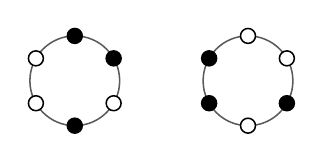
\begin{tikzpicture}[line width=.55pt]
\draw[black!65] (0,0) circle (0.57cm);
\foreach \i/\shade in {0/black,1/black,2/white,3/black,4/white,5/white}
  \filldraw[fill=\shade] (90-60*\i:0.57cm) circle (2.7pt);
\begin{scope}[xshift=2.2cm]
\draw[black!65] (0,0) circle (0.57cm);
\foreach \i/\shade in {0/white,1/white,2/black,3/white,4/black,5/black}
  \filldraw[fill=\shade] (90-60*\i:0.57cm) circle (2.7pt);
\end{scope}
\end{tikzpicture}\par
{\small The six-bead word $110100$ and its reverse have disjoint sets of rotations.\\
Repeating either word three times produces the same twelve-element orbit at length 18.}
\end{center}


\newpage
\section{The lengths at which the original rule fails}
Hadjicostas's proposed rule for $1\le k\le n$ uses $b(n)$, the number of bracelets that are imprimitive or achiral. Let $\mu$ denote the Möbius function. The prediction is
\begin{equation}\label{eq:pred}
 T(n,k)=
 \begin{cases}
 \sum_{d\mid k}\mu(d)b(k/d),& k\mid n,\\
 0,& k\nmid n .
 \end{cases}
\end{equation}
\begin{theorem}\label{th:fail}
A binary row disagrees with \eqref{eq:pred} exactly when $n$ has an odd divisor $t\ge3$ with $n/t\ge6$. The nonzero entries at a nondivisor $k\le n$ occur precisely at $k=2n/t$ for these $t$, where their value is $C_2(n/t)$. The complete set of agreeing lengths is
\[
 \{2^a:a\ge0\}\ \cup\ \{p,2p,4p:p\text{ an odd prime}\}\ \cup\ \{9,15,25\}.
\]
\end{theorem}
\begin{proof}
A primitive chiral binary bracelet exists in every length $p\ge6$. Take three ones whose successive cyclic gaps of zeros are $0,1,p-4$. The gaps are distinct, so no nonidentity cyclic shift or reversal of this gap triple preserves it. The word is therefore primitive and chiral. For $p\le5$ the minority color occurs at most twice. A reflection can fix one position or exchange any specified two positions, so every binary bracelet is achiral.

By Theorem~\ref{th:entries}, $k\nmid n$ with $k\le n$ can occur only as $k=2p$ for $p\mid n$, $p\ge6$, with the quotient $t=n/p$ odd and at least three. This proves the assertion about nondivisors. If there is no such $t$, the same holds at every divisor $m$ of $n$. Indeed any witness $p\mid m$ with odd repetition factor $t$ gives $n/t\ge m/t\ge6$. For $k\mid m$, Theorem~\ref{th:entries} gives a value independent of $m$, namely $D(k)=R_2(k)+\one_{2\mid k}C_2(k/2)$, with the second term omitted for odd $k$. The sole additional possible size is $2m$, counting exactly the primitive chiral bracelets omitted from $b(m)$. Consequently $b(m)=\sum_{k\mid m}D(k)$ for every $m\mid n$. Möbius inversion gives \eqref{eq:pred} also at the divisor columns. In the other direction a positive entry at a nondivisor contradicts \eqref{eq:pred}.

If $n$ has an odd prime divisor, choose the smallest one, $p$. The criterion says that the row agrees precisely when $n/p\le5$. A cofactor $1,2$ or $4$ gives $p,2p,4p$. If the cofactor is $3$ or $5$, the minimality of $p$ gives $9,15$ or $25$. Every power of two also agrees.
\end{proof}

The union is disjoint. Writing $\pi_o(x)$ for the number of odd primes up to $x$, its counting function for $x\ge1$ is
\[
 1+\lfloor\log_2 x\rfloor+\pi_o(x)+\pi_o(x/2)+\pi_o(x/4)
           +\one_{x\ge9}+\one_{x\ge15}+\one_{x\ge25}.
\]
The prime number theorem gives $7x/(4\log x)$ as the leading asymptotic. The disagreeing rows therefore have natural density one.

\newpage
\section{Evaluation and prior work}\label{sec:count}
For any $q\ge2$ define
\[
 F_q(d)=\begin{cases}q^{(d+1)/2},& d\text{ odd},\\
 (q+1)q^{d/2}/2,& d\text{ even}.
 \end{cases}
\]
The standard primitive counts needed in Theorem~\ref{th:entries} take the form
\begin{align*}
 L_q(p)&=\frac1p\sum_{d\mid p}\mu(d)q^{p/d},
 &R_q(p)&=\sum_{d\mid p}\mu(d)F_q(p/d),
 &C_q(p)&=\frac{L_q(p)-R_q(p)}2 .
\end{align*}
Here $L_q$ counts primitive rotational necklaces. Counting words by least period and applying Möbius inversion gives its numerator, and each primitive necklace has $p$ words. To see the formula for $R_q$, count pairs consisting of a word of length $d$ and a reflection fixing it. An achiral necklace of period $e$ has $e$ distinct words. Each has $d/e$ fixing reflections, since those reflections form a coset of its rotational stabilizer. Thus the total pair count divided by $d$ counts all achiral necklaces. For odd $d$ every reflection fixes one position and exchanges the other positions in pairs. For even $d$ half the reflections fix two positions and half fix none. The resulting count is $F_q(d)$. Inverting over all possible primitive periods gives $R_q$. Pairing the remaining primitive necklaces by reversal gives $C_q$. For two colors, averaging rotations and reflections gives the total bracelet count $F_2(n)/2+(2n)^{-1}\sum_{d\mid n}\varphi(d)2^{n/d}$. Subtracting $C_2(n)$ gives $b(n)$, including the small lengths.

At $n=18$, $C_2(6)=1$, $C_2(9)=14$ and $R_2(18)=728$. At $n=21$, $C_2(7)=2$ and $R_2(21)=2030$. These account for both examples already reported by Hadjicostas.
\begin{center}
\begin{tabular}{@{}rrrr@{}}\toprule
$n$ & $k$ & Prediction \eqref{eq:pred} & $T(n,k)$\\\midrule
18 & 12 & 0 & 1\\
18 & 18 & 743 & 742\\
21 & 14 & 0 & 2\\
21 & 21 & 2032 & 2030\\\bottomrule
\end{tabular}
\end{center}

A third color moves the threshold. For every $q\ge3$ and $p\ge3$, the word $0^{p-2}12$ is primitive because the symbol $1$ occurs once. A reflection preserving it would fix both adjacent, uniquely colored positions, which is impossible for $p\ge3$. Lengths 1 and 2 have only achiral bracelets. The same proof gives the analogous divisor rule for $q\ge3$ precisely on the powers of two, the odd primes and twice the odd primes.

The primitive counts above have earlier treatments in the OEIS and Hadjicostas's work on chirality and co-periods. The row classification applies those counts to the refinement requested in \oeis{203399}. The accompanying \texttt{verify.py} exhausts every binary word through length 21 and every ternary word through length 9. It also checks the original and corrected row formulas against each other through length 1000.

\smallskip
{\small
\noindent\textbf{Sources.}
G. Critzer and P. Hadjicostas, \oeis{203399}, especially the June 2019 formula and counterexamples.
P. Hadjicostas, \href{https://oeis.org/A203399/a203399.pdf}{\emph{On the number of aperiodic chiral bracelets of two colors}} (2019), and \href{https://doi.org/10.54550/ECA2023V3S3R23}{\emph{On the Number of Bracelets Whose Co-periods Divide a Given Integer}}, Enumerative Combinatorics and Applications 3:3 (2023), Article S2R23.
See also \oeis{032239}, \oeis{056493}, and \href{https://dlmf.nist.gov/27.12}{NIST DLMF, \S27.12} for the prime number theorem.}
\end{document}
